\documentclass[12pt,a4paper,titlepage]{article}
\usepackage[utf8]{inputenc}
\usepackage[top=3cm, bottom=3cm, left=2cm, right=2cm]{geometry}
\usepackage{amsmath}
\usepackage{amsfonts}
\usepackage{amssymb}
\usepackage{fancyhdr}
\usepackage{lastpage}
\usepackage{fix-cm}
\usepackage{graphicx}
\usepackage{hyperref}
\usepackage{color}
\usepackage{mdwlist}
\usepackage{listings}
\usepackage[perpage,para,bottom]{footmisc}
\setlength{\headheight}{30pt}
\pagestyle{fancy}
\renewcommand{\figurename}{Abb}
\renewcommand{\contentsname}{Inhaltsverzeichnis}
\renewcommand{\listfigurename}{Liste der Abbildungen}

\lhead{Nicolas Hafner 6S}
\chead{Transcend}
\rhead{Zürich, Dezember 2011}
\cfoot{\thepage\ / \pageref{LastPage}}
\lfoot{\copyright 2011 TymoonNET/NexT}

\author{Nicolas Hafner}
\title{Transcend}

\begin{document}
\begin{titlepage}
\begin{center}
	Maturitätsarbeit an der Kantonsschule Oerlikon  \\
	\vskip 2cm
	
\includegraphics[keepaspectratio=true,scale=0.5,bb=0 0 1024 256]{logo.png}
	\vskip 0.5cm
	\begin{Large}Engineprogrammierung und Gamedesign von Grund auf\end{Large}\\
	\vskip 1cm
	Erstellt und Konzipiert von Nicolas Hafner, 6S\\
	Betreut von Clemens Holenstein\\
	\vskip 0.5cm
	Zürich, Dezember 2011
\end{center}
\end{titlepage}

\tableofcontents
\listoffigures

\newpage

\section{Einführung}
	\subsection{Idee}
		Ich hatte schon früh in meiner Jugend Interesse daran, Spiele selbst zu erstellen.
		So hielt ich oft Ausschau nach Spielen, die einen Level Editor beinhalteten, damit ich mit diesem meine eigenen Welten erstellen konnte.
		Es dauerte auch nicht lange bis ich auf die Idee kam eigene Spiele von Grund auf zu bauen, und bin so auf GameMaker gestossen.
		GameMaker ist ein vereinfachtes Tool zur Erstellung von Videospielen. Allerdings gibt es auch bei diesem Programm relativ grosse Einschränkungen.
		Es brachte mir aber dennoch einen Einstieg in die Welt des Gamedesigns und ich habe einige Spiele erstellt, von welchen aber keines je fertiggestellt wurde oder auch irgendwie Nennenswert wäre.\\
		
		Auf meiner suche nach mehr Möglichkeiten habe ich mich dann irgendwann entschieden eine richtige Programmiersprache zu lernen und bin so auf Java gestossen, welches ich nun seit vielen Jahren extensiv gebrauche und schon etliche Programme damit erstellt habe.
		Es war mir deshalb schon Jahre vorher klar, dass ich für die Maturarbeit ein Programm schreiben würde.
		Was es genau sein würde, wusste ich aber lange noch nicht. Ich hatte ursprünglich viele Ideen, wie z.B. einen Raytracer\footnotemark, einen Fraktal Generator/Animator\footnotemark, oder einen Simulator für Neuronale Netze\footnotemark.\\
		
		Allerdings habe ich vor etwas mehr als Zweieinviertel Jahren angefangen zu Zeichnen, und das Programmieren ist für einige Zeit in den Hintergrund gerutscht.
		Heute habe ich eine Balance von beidem erreicht. Durch das neu gefundene Interesse im eher künstlerischen Bereich haben sich aber auch meine Ziele und Absichten verändert.
		Als sich nun die Frage der Maturarbeit offenbarte war mir klar, dass ich etwas finden müsste, das beide Aspekte, sowohl das Zeichnerische als auch das Programmiertechnische, beinhaltet.\\
		Ich hatte auch bis dann noch nicht die Sehnsucht, ein eigenes Spiel zu erstellen, verloren. Nur war die Zeit oft knapp und ich hatte bereits viele andere Projekte die meine Freizeit in Anspruch nahmen. Die Erstellung eines Spiels nimmt enorm viel Zeit in Anspruch. Zeit, die ich sonst nicht hatte.\\
		
		Da ich aber so oder so einige Zeit in die Maturarbeit investieren müsste, war es nicht weit hergeholt, das Thema meiner Maturarbeit um die Spielprogrammierung und das allgemeine Gamedesign zu setzen. So hätte ich endlich genug Zeit eingeräumt, im etwas anständiges zu produzieren.
		Das Ziel war es damals, ein möglichst weit entwickeltes Spiel zu produzieren, damit ich auch endlich mal etwas richtiges zu zeigen hätte und auch etwas gemacht hätte, worauf ich stolz sein könnte.
		
		\footnotetext[1]{Ein Raytracer erzeugt ein zweidimensionales Bild einer dreidimensionaler, digitaler Szene durch Anwendung von physikalischen Eigenschaften, Berechnungen und Verfahren. Raytracing ist ein sehr breites und komplexes Feld der Informatik und ist stark mit Mathematik und Physik verbunden.}
		\footnotetext[2]{Ein Fraktal Generator errechnet und färbt einen Ausschnitt eines Fraktals. Dabei kann der Benutzer den Ausschnitt frei wählen und sich im Fraktal bewegen.}
		\footnotetext[3]{Simulatoren für Neuronale Netze sind der Versuch, ein Gehirn, oder zumindest die Art wie das Gehirn lernt mit Software zu repräsentieren und so eine künstliche, lernende Intelligenz zu erstellen.}
		
	\subsection{Übersicht}
		Normalerweise werden Spiele in Teams erstellt, wo meistens eine grosse Menge and Spezialisten am Werk sind und miteinander kooperieren, Ideen bringen und ihr Wissen mit einfliessen lassen.
		Dies ist vor allem so, da Game Design und Speileerstellung ein enormes Gebiet ist, welches viele verschiedene Bereiche anspricht.
		\begin{figure}[h!]
  			\centering
			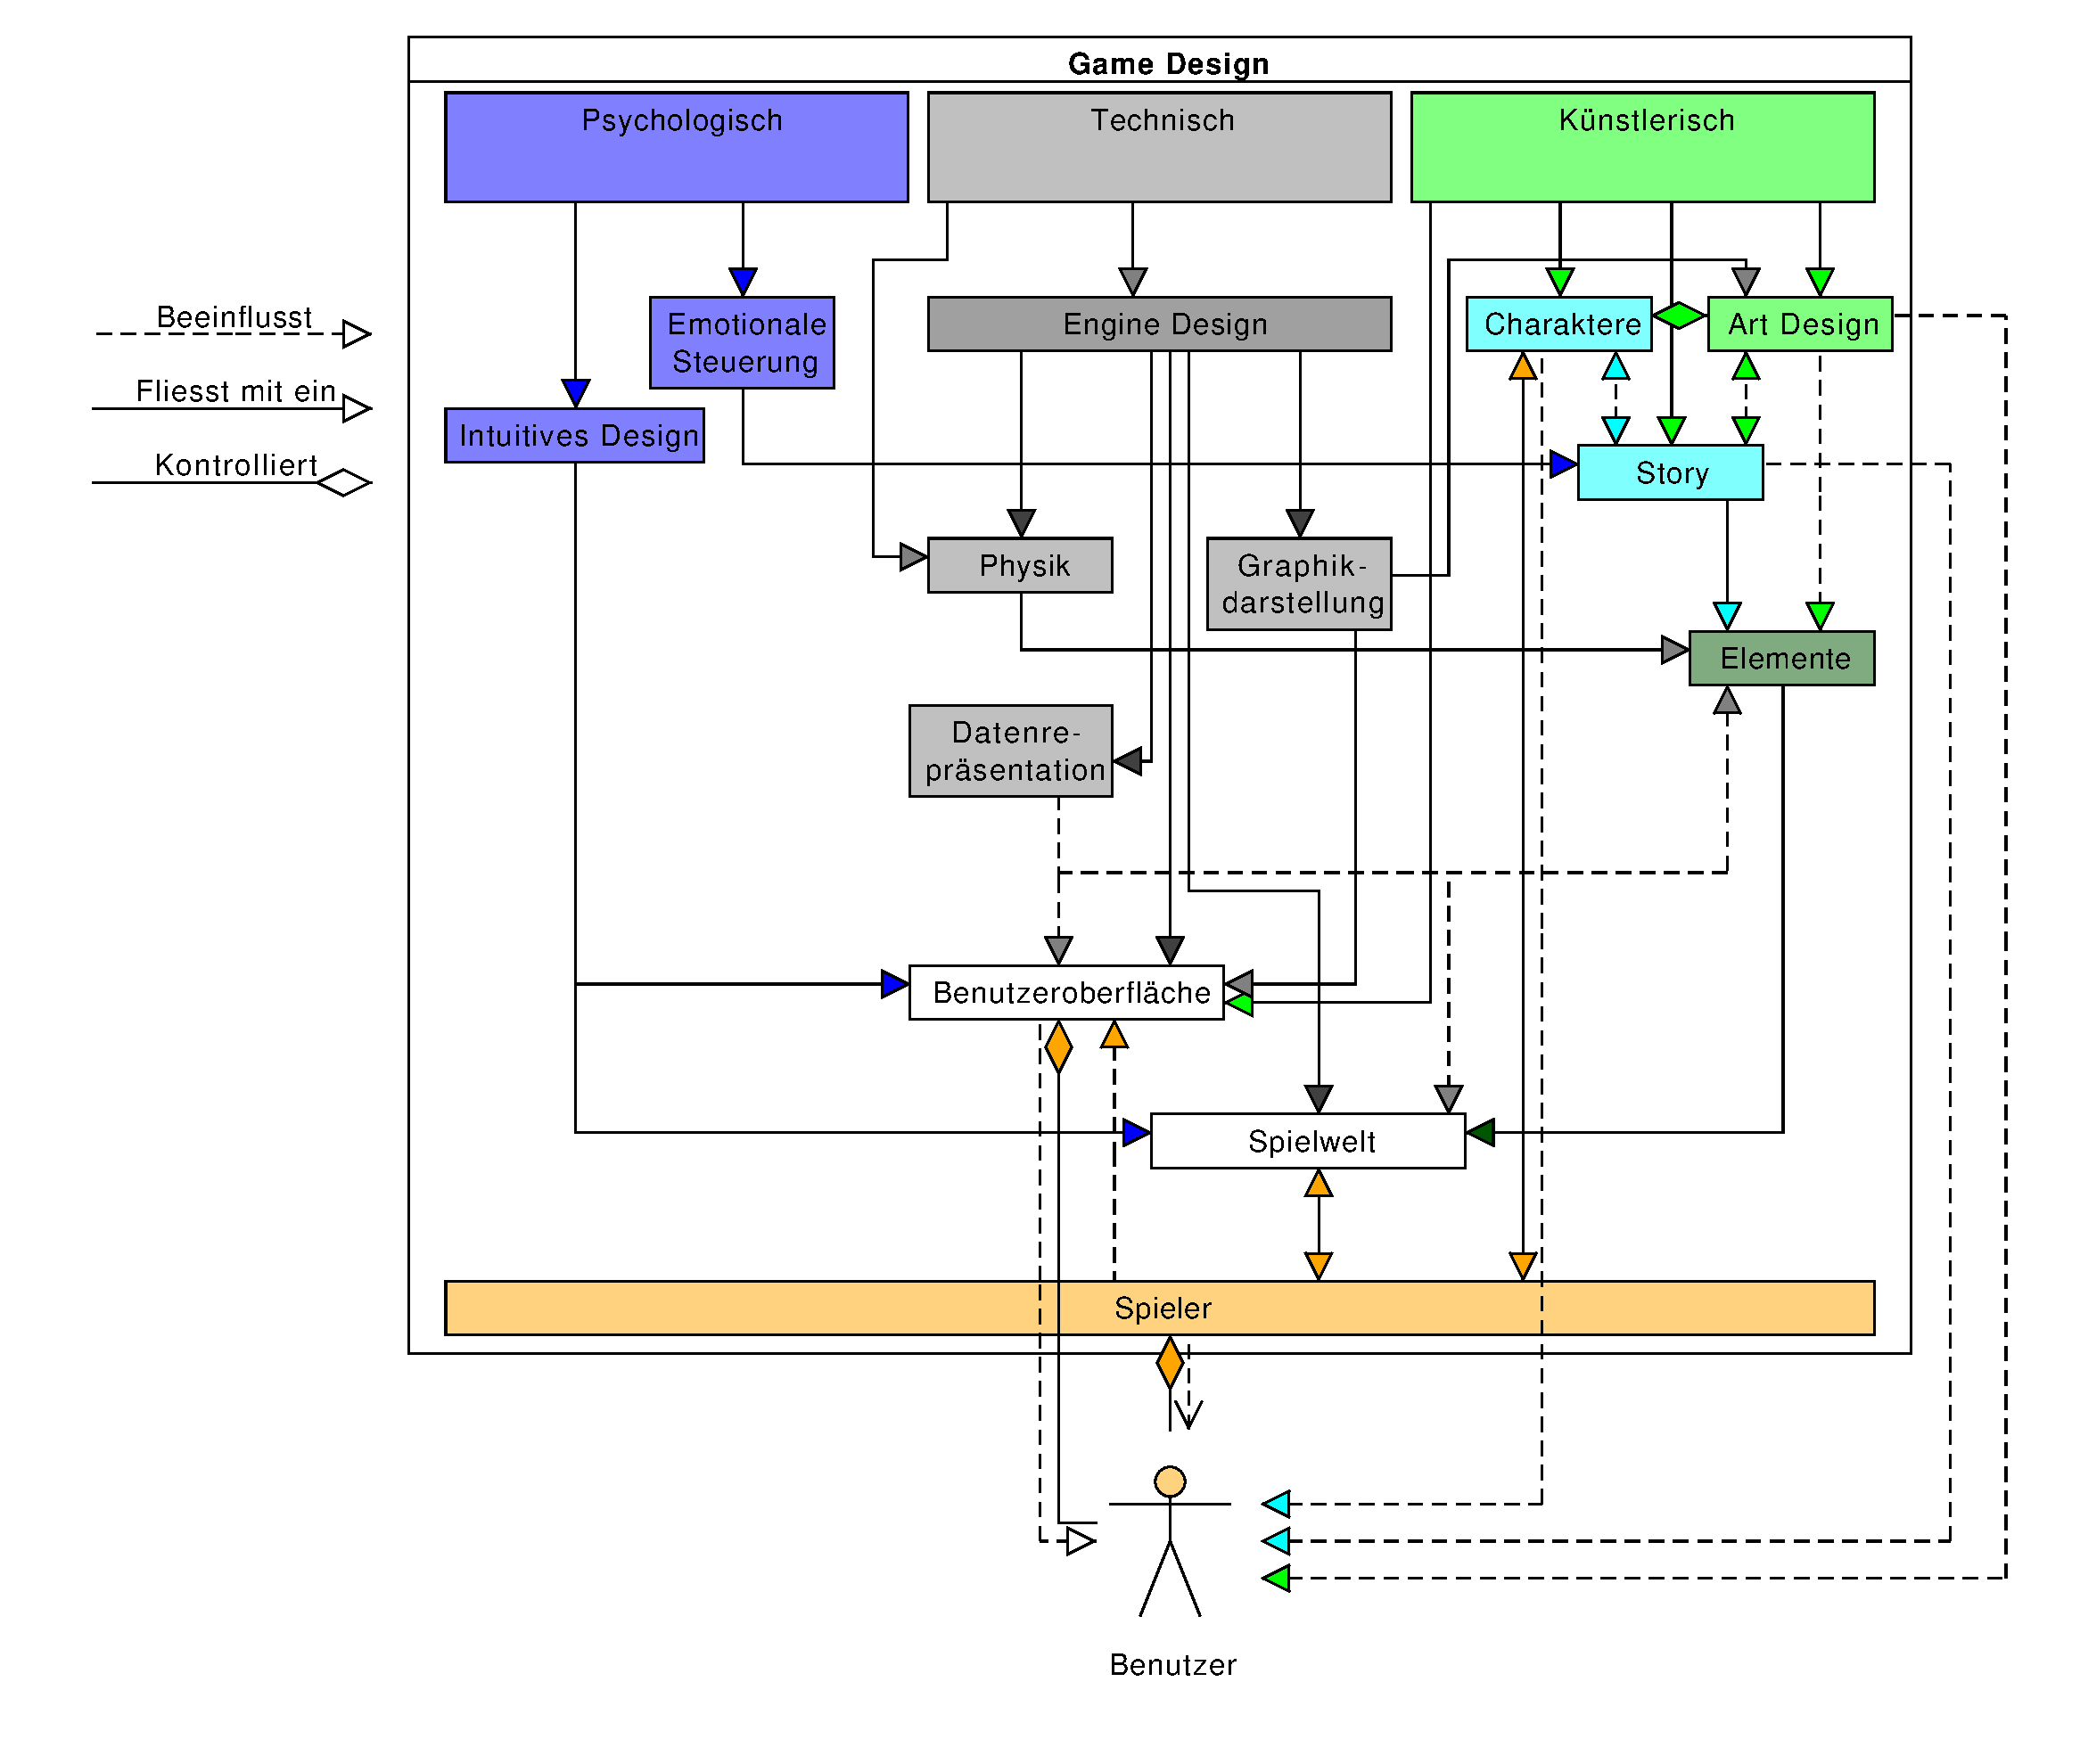
\includegraphics[keepaspectratio=true,scale=0.4]{gamedesign.pdf}
  			\caption{Darstellung einiger Bereiche des Game Designs}
		\end{figure}
		Um alle diese Bereiche zu decken ist ein enormes Wissen notwendig. Viele der Bereiche können auch nur durch ständiges Ausprobieren und Testen perfektioniert werden, was viel Zeit beansprucht.\\
		
		In meiner Arbeit habe ich mich vor allem auf das Technische konzentriert, versuchte aber dennoch auf die anderen Bereiche einzugehen und habe mich ausgiebig über sie Informiert.\\
		Auch wenn im praktischem Produkt nicht auf alles eingehen werden konnte, da es aus zeitlichen Gründen nicht reichte, wird dennoch auf all diese Aspekte in diesem Dokument eingegangen.
		Dabei handelt es sich um Psychologische, Anthropologische, Mathematische, Physikalische, Künstlerische und Musische Überlegungen und Konzepte, die alle beim Game Design eine rolle spielen.
		
	
	\subsection{Konzepte}
		%What kind of elements, ideas and concepts did I originally have
		Als ich mit dem Projekt begann habe ich mir vor allem Dinge überlegt, die erst sehr spät im Prozess zum Einsatz kämen. So hatte ich Ideen für Spielkonzepte, eine Story und einige Grundcharaktere. 
		Das Wichtigste dabei war mir, dass das Spiel in 2D war und einen Jump \& Run Ansatz wie z.B. Super Mario oder Sonic the Hedgehog verfolgte.
		Allerdings ist dies ja nicht eine so originelle Idee, weshalb ich mir einige Spezialitäten überlegen musste.\\
		
		Auf der Suche nach neuen Ansätzen dachte ich zurück an Spiele, die mir selbst sehr gut gefielen. Am stärksten trat dabei Okami\footnote{\url{www.okami-game.com/}} hervor. Daraus habe ich auch das Konzept der Fähigkeiten übernommen. Damit meine ich, dass der Spieler über den Verlauf des Spiels neue Fähigkeiten erlangt, die er dann benutzen kann um neue Regionen in der Welt zu erreichen, die er vorher noch nicht erreichen konnte. Dies ist im starken Kontrast zu herkömmlichen J\&Rs, wo einem alle Fähigkeiten (bis auf Power-ups) von Beginn an verfügbar sind. Des weiteren erlaubt dieses Konzept einen weitaus grösseren Grad an Komplexität und Wiederspielbarkeit. So steht dem Spieler die ganze Welt von Anfang an offen, was ihm erlaubt sie ausgiebig auszukundschaften und sich schon im voraus Gedanken zu machen, was später einmal möglich sein wird oder interessant wäre.\\
		
		Im Unterschied zu Okami, in welchem die Fähigkeiten nur limitierten Einfluss haben, war die Idee bei mir, dass jede Fähigkeit seine eigenen Vorteile und Nachteile bringen sollte, um den Spieler mehr zum denken anzuregen. So kam ich auf den Schluss, dass es am interessantesten wäre, dieses Konzept mittels Formen einzuführen.
		

\section{Enginedesign \& Programmierung}
	\subsection{Einführung}
		%Engine is core part, handles resources and so on.
		%Does base calculations, is what makes the game run.
		%Abstraction layers between core engine and game engine
		
	\subsection{Techniken \& Tools}
		%Explanation of OGL/AL, LWJGL, etc.
		%Thoughts about loading resources, resource management and sharing.
		
	\subsection{Ziele \& Einsatzmöglichkeiten}
		%Base 2D environments
		%2D games
		
	\subsection{Codedesign}
		%UML Diagrams
		
	\subsection{Probleme im Detail}
		%Small intro text
		
		\subsubsection{Kollisionserkennung}
			%You know what to do in these parts
			%Diagrams
			
		\subsubsection{AI}
			%Diagrams
			
		\subsubsection{Events \& GUI}
			%Diagrams
			

\section{Grafikdesign}
	\subsection{Einführung}
		%Which parts does graphics design cover
		
	\subsection{Ideen \& Konzepte}
		%Which thoughts have I given the character design
		%How is it incorporated in the story
		
	\subsection{Einschränkungen}
		%Limitations by the engine
		%Time like limitations and speedups

\section{Gamedesign}
	\subsection{Einführung}
		%What is game design, how does it flow together?
		%What skills do you need for this?
		
	\subsection{Charakterdesign}
		%What is important for characters?
		%How do they relate tothe artwork and story?
		%What was my implementation of this, what though path did I take?
		
	\subsection{Spielmechaniken}
		%What are game mechanics?
		%How do they get planned, what do you have to think about?
		%What kind of mechanics did I incorporate?
		
	\subsection{Story}
		%Is a story relevant or necessary?
		%How does a story intervine with everything else?
		%The story I planned for this
		
	\subsection{Leveldesign}
		%Level design specialities
		%What a level designer has to think about
		%Difficulties of level design
	
\section{Schlussfolgerung \& Aussicht}
	\subsection{Schlussfolgerungen}
		%What problems were most annoying?
		%How far did I actually come
		%What do I think of my progress
		%How should I have re-scheduled?
		
	\subsection{Erweiterungsmöglichkeiten}
		%What am I going to do with this still?
		%Other things I could extend on
		
\clearpage
\section{Danksagung, Referenzen \& Weiteres}
	\subsection{Persönlicher Dank}
		%People that are fucking awesome and helped me
		Über die Zeit, die ich an dieser Arbeit verbracht habe, habe ich mit einigen Personen immer wieder Ideen und Konzepte diskutiert, anfällige Probleme bearbeitet und nach neuen Ansätzen gesucht (und zum Teil, wenn es aussichtslos schien, holte ich mir auch emotionale Unterstützung bei ihnen).
		Ich möchte all diesen Personen meinen grössten Dank verrichten und bin mir sicher, dass ich ohne sie diese Arbeit nie so weit gebracht hätte oder überhaupt erst auf diese Idee gekommen wäre.\\
		\newline
		Als erstes möchte ich Herrn Clemens Holenstein für eine gute Betreuung und nahtloses Zusammenarbeiten bei der Maturarbeit bedanken. Ich bin über alles froh, dass ich dieses Thema wählen durfte und er mir die Freiheit gegeben hat, die ich benötigte um diese Arbeit anzugehen.\\
		\newline
		Des Weiteren danke ich Frau Tanja Dorigo für die Zustimmung die Rolle der Zweit-Bezugsperson zu übernehmen. Ausserdem bedanke ich mich für eine sehr informative und fördernde Diskussionsstunde, die wir zusammen geführt haben.\\
		\newline
		Obwohl Herr Michael Stadelmann nicht mehr an unserer Schule ist, so danke ich ihm für das ursprüngliche Anspornen und die Überzeugungskraft, dass ich dieses Projekt auch in angriff nehmen könne, die er mir gegeben hat.\\
		\newline
		Selbstverständlich bin ich sehr froh über die Unterstützung, die mir meine Familie und meine Klassenkameraden gegeben haben, und das Interesse, das sie an meiner Arbeit gezeigt haben. Auch dafür möchte ich meinen Dank aussprechen, und hoffe dass sie auch weiterhin Interesse an der Weiterführung meiner Arbeit zeigen werden.\\
		\newline
		Speziell möchte ich noch Yassin Sdiri erwähnen, der mir als lang bekannter Freund auch oft zur Seite gestanden ist und mir auch seine Hilfe angeboten hat.\\
		\newline
		Weiterhin danke ich Malakin, welcher mir bei einigen Problemen im technischen Bereich mit seinem Know-How zur Hilfe kam und mir auch oft geholfen hat grobe Fehler in den Konzepten auszumerzen.\\
		\newline
		Ich möchte auch all meinen anderen Freunden, die ich nur über das Internet erreichen kann, danken und hoffe auf eine lange Bekanntschaft und Zusammenarbeit.\\
		\newline
		Schlussendlich will ich an dieser Stelle all jenen Danken, die an den Projekten und Büchern gearbeitet haben, die ich für diese Arbeit benutzt habe. Es wäre ohne ihre Vorarbeit und Bemühung nie für mich möglich gewesen auch nur mit der Arbeit zu beginnen. Sie haben den Grundstein und die Grundwerkzeuge bereitgestellt, die nötig waren um mir eine zielgerichtete und produktive Arbeitsumgebung zu ermöglichen.\\
		
	\subsection{Tools, Webseiten \& Bücher}
		\paragraph{Programme, Libraries \& Tools}
		\begin{itemize*}
			\item \href{http://jdk6.java.net/}{Sun Java 6 JDK} \url{http://jdk6.java.net/}
			\item \href{http://www.lwjgl.org/}{LightWeight Java Game Library (OpenGL \& OpenAL)} \url{http://www.lwjgl.org/}
			\item \href{http://slick.cokeandcode.com/}{Slick-Util (Teil von Slick2D)} \url{http://slick.cokeandcode.com/}
			\item \href{http://tymoon.eu}{TymoonNET/NexT library} \url{http://tymoon.eu}
			\item \href{http://netbeans.org/}{NetBeans IDE 6.9} \url{http://netbeans.org/}
			\item \href{http://git-scm.com/}{GIT Version Control} \url{http://git-scm.com/}
			\item \href{http://www.syntevo.com/smartgit/}{SmartGIT GIT Client} \url{http://www.syntevo.com/smartgit/}
			\item \href{http://www.systemax.jp/en/sai/}{Paint Tool SAI} \url{http://www.systemax.jp/en/sai/}
			\item \href{http://www.adobe.com/products/photoshop.html}{Adobe Photoshop CS3} \url{http://www.adobe.com/products/photoshop.html}
			\item \href{http://www.renoise.com/}{Renoise} \url{http://www.renoise.com}
			\item \href{http://audacity.sourceforge.net/}{Audacity} \url{http://audacity.sourceforge.net/}
		\end{itemize*}
		\paragraph{Webseiten}
		\begin{itemize*}
			\item \href{http://www.stackoverflow.com}{Stack Overflow} \url{http://www.stackoverflow.com}
			\item \href{http://gamedev.stackexchange.com/}{Stack Exchange/Gamedev} \url{http://gamedev.stackexchange.com/}
			\item \href{http://download.oracle.com/javase/6/docs/api/}{Java 6 javadoc} \url{http://download.oracle.com/javase/6/docs/api/}
			\item \href{http://www.lwjgl.org/forum/}{LWJGL Forum} \url{http://www.lwjgl.org/forum/}
		\end{itemize*}
		\paragraph{Bücher}
		\begin{itemize*}
			\item \href{http://artofgamedesign.com/}{The Art of Game Design (Englisch)} \url{http://artofgamedesign.com/}
			\item \href{http://www.opengl.org/documentation/red_book/}{OpenGL The Red Book (Englisch)} \url{http://www.opengl.org/documentation/red_book/}
		\end{itemize*}
		
\end{document}